\chapter{Описание структуры и архитектуры проекта}\label{ch:ch4}
\section{Диаграмма развёртывания}\label{sec:ch4/sect1}
На рисунке~\ref{fig:overview_components_diagram} показана диаграмма развёртывания приложения.
\begin{figure}[ht]
  \centerfloat{
    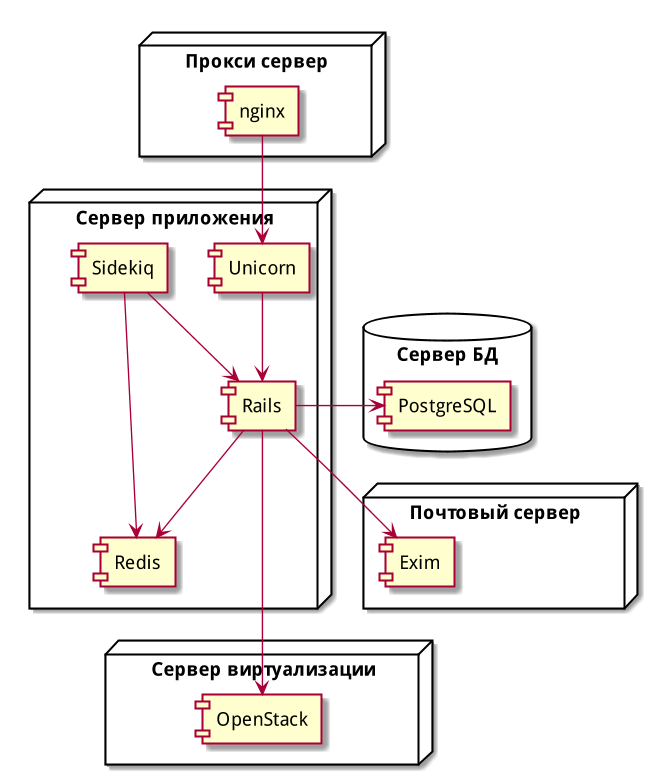
\includegraphics[scale=0.4]{umls/overview_components_diagram}
  }
  \caption{Диаграмма развёртывания.}\label{fig:overview_components_diagram}
\end{figure}

\section{Описание компонентов}\label{sec:ch4/sect2}
Приложение на Rails использут архитектуру сервисных объектов (Service Objects), которая заключается в использовании отдельных классов для инкапсуляции сложных процессов. Такие классы имеют имеют простой интерфейс, позволяющий приложению испоьзовать их как черный ящик. Экземпляры подобных классов энкапсулирует логику с данными одного определённого процесса.


Каждый компонент представляет из себя модуль с сервисными классами, которые выполняют определённую работу связанную с их компонентом.


На рисунке~\ref{fig:application_scheme} показана общая диаграмма компонентов приложения.
\begin{figure}[ht]
  \centerfloat{
    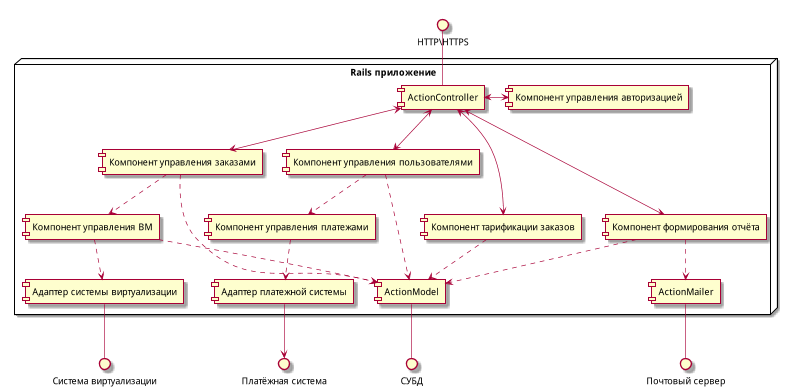
\includegraphics[scale=0.6]{umls/application_scheme}
  }
  \caption{Диаграмма компонентов приложения}\label{fig:application_scheme}
\end{figure}

\subsection{Компонент управления заказами}\label{sec:subs1}
Данный компонент, модуль, отвечает за все действия с заказами, включая проверку параметров и работы с адаптером системы виртуализации.
Каждое действие имеет свой модуль, в котором уже находятся классы для операций.

При оформлении заказа вызывается эндпоинт модуля создания заказа, который вызывает контракт проверяющий параметры, после чего сохраняет заказ в статусе "Создаётся" и отправляет сигнал разворачивания ВМ в сервис создания ВМ.

При завершении разворачивания ВМ в компонент придёт запрос на изменение состояния заказа.

На рисунке~\ref{fig:order_control_scheme} показана диаграмма компонента управления заказами.
\begin{figure}[ht]
  \centerfloat{
    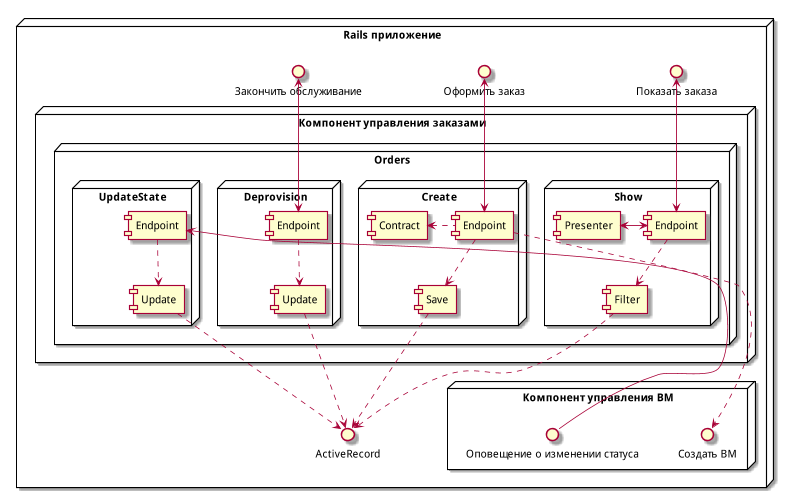
\includegraphics[scale=0.6]{umls/order_control_scheme}
  }
  \caption{Диаграмма компонента управления заказами}\label{fig:order_control_scheme}
\end{figure}

\subsection{Компонент управления ВМ}\label{sec:subs2}
\subsection{Компонент управления пользователями}\label{sec:subs3}
\subsection{Компонент формирования отчётов}\label{sec:subs4}
\subsection{Компонент тарификации заказов}\label{sec:subs5}


\section{Концептуальная модель базы данных}\label{sec:ch4/sect3}

% \section{Компонент управления заказами}\label{sec:ch4/sect1}


% \section{Компонент управления заказами}\label{sec:ch4/sect1}
% \section{Компонент формирования отчётов}\label{sec:ch4/sect2}
% \section{Компонент работы с системой виртуализации}\label{sec:ch4/sect3}
% \section{Компонент тарификации заказов}\label{sec:ch4/sect4}

% \section{Диаграммы вариантов использования}\label{sec:ch4/sect1}
% \subsection{Создание аккаунта пользователя}\label{sec:subs12}
% \subsection{Создание заказа}\label{sec:subs13}
% \subsection{Управление заказом}\label{sec:subs14}

% \section{Диаграммы последовательностей}\label{sec:ch4/sect2}
% \subsection{Создание аккаунта пользователя}\label{sec:subs21}
% \subsection{Создание заказа}\label{sec:subs22}
% \subsection{Управление заказом}\label{sec:subs23}

% \section{Диаграмма состояний объектов системы}\label{sec:ch4/sect3}
% \subsection{Аккаунт пользователя}\label{sec:subs31}
% \subsection{Заказ}\label{sec:subs32}

% \section{Концептуальная модель базы данных}\label{sec:ch4/sect4}
% \section{Архитектура системы(?)}\label{sec:ch4/sect5}
